% =============================================================================
% Sensitivity Analysis - Parallel AVL Trees
% Technical Report
% Author: Lucas Sotomayor
% =============================================================================

\documentclass[11pt,a4paper]{article}

\usepackage[utf8]{inputenc}
\usepackage[T1]{fontenc}
\usepackage[english]{babel}
\usepackage{amsmath,amssymb}
\usepackage{booktabs}
\usepackage{multirow}
\usepackage{graphicx}
\usepackage{xcolor}
\usepackage{listings}
\usepackage{geometry}
\usepackage{fancyhdr}
\usepackage{hyperref}
\usepackage{float}
\usepackage{caption}
\usepackage{subcaption}
\usepackage{pgfplots}
\pgfplotsset{compat=1.18}

\geometry{margin=1in}

% Colors
\definecolor{codegreen}{rgb}{0,0.6,0}
\definecolor{codegray}{rgb}{0.5,0.5,0.5}
\definecolor{codepurple}{rgb}{0.58,0,0.82}
\definecolor{backcolour}{rgb}{0.95,0.95,0.92}

% Listings style
\lstdefinestyle{mystyle}{
    backgroundcolor=\color{backcolour},
    commentstyle=\color{codegreen},
    keywordstyle=\color{blue},
    numberstyle=\tiny\color{codegray},
    stringstyle=\color{codepurple},
    basicstyle=\ttfamily\small,
    breaklines=true,
    numbers=left,
    frame=single
}
\lstset{style=mystyle}

% Header
\pagestyle{fancy}
\fancyhf{}
\rhead{Parallel AVL Trees}
\lhead{Sensitivity Analysis}
\rfoot{Page \thepage}

\title{
    \textbf{Sensitivity Analysis of Configuration Parameters} \\
    \large Production-Grade Parallel AVL Trees \\
    \vspace{0.5cm}
    \normalsize Technical Report
}
\author{Lucas Sotomayor \\ R\&D Division}
\date{\today}

\begin{document}

\maketitle

\begin{abstract}
This technical report presents a systematic sensitivity analysis of the configuration parameters in the Parallel AVL Tree implementation. We analyze 8 key parameters across 4 workload types, measuring their impact on balance score, throughput, redirect behavior, and attack resistance. Our findings validate the default configuration while identifying optimal values for specific use cases including high-security and high-performance scenarios.
\end{abstract}

\tableofcontents
\newpage

% =============================================================================
\section{Introduction}
% =============================================================================

The Parallel AVL Tree implementation contains several configurable parameters that control routing behavior, hotspot detection, anti-thrashing mechanisms, and rebalancing policies. Understanding the sensitivity of system performance to these parameters is critical for:

\begin{itemize}
    \item \textbf{Production deployment}: Selecting optimal values for specific workloads
    \item \textbf{Security hardening}: Tuning parameters for adversarial resistance
    \item \textbf{Performance optimization}: Maximizing throughput under normal conditions
    \item \textbf{Validation}: Confirming that default values are reasonable
\end{itemize}

% =============================================================================
\section{Parameters Under Analysis}
% =============================================================================

\subsection{Router Parameters}

\begin{table}[H]
\centering
\caption{Router Configuration Parameters}
\begin{tabular}{@{}llll@{}}
\toprule
\textbf{Parameter} & \textbf{Default} & \textbf{Type} & \textbf{Location} \\
\midrule
\texttt{VNODES\_PER\_SHARD} & 16 & size\_t & router.hpp \\
\texttt{WINDOW\_SIZE} & 50 & size\_t & router.hpp \\
\texttt{HOTSPOT\_THRESHOLD} & 1.5 & double & router.hpp \\
\texttt{MAX\_CONSECUTIVE\_REDIRECTS} & 3 & size\_t & router.hpp \\
\texttt{REDIRECT\_COOLDOWN} & 100ms & duration & router.hpp \\
\bottomrule
\end{tabular}
\end{table}

\subsection{Cache Parameters}

\begin{table}[H]
\centering
\caption{CachedLoadStats Configuration}
\begin{tabular}{@{}llll@{}}
\toprule
\textbf{Parameter} & \textbf{Default} & \textbf{Type} & \textbf{Location} \\
\midrule
\texttt{refresh\_interval} & 1ms & duration & cached\_load\_stats.hpp \\
\bottomrule
\end{tabular}
\end{table}

\subsection{Architecture Parameters}

\begin{table}[H]
\centering
\caption{ParallelAVL Architecture Configuration}
\begin{tabular}{@{}llll@{}}
\toprule
\textbf{Parameter} & \textbf{Default} & \textbf{Type} & \textbf{Location} \\
\midrule
\texttt{num\_shards} & 8 & size\_t & parallel\_avl.hpp \\
\texttt{rebalance\_threshold} & 2.0 & double & AVLTreeParallel.h \\
\texttt{balance\_score\_min} & 0.8 & double & AVLTreeParallel.h \\
\bottomrule
\end{tabular}
\end{table}

% =============================================================================
\section{Methodology}
% =============================================================================

\subsection{Workload Characterization}

We test each parameter configuration against four distinct workloads:

\begin{enumerate}
    \item \textbf{Uniform}: Keys drawn uniformly at random from $[0, 100000]$
    \item \textbf{Zipfian}: Power-law distribution with $\alpha = 0.99$ (80/20 rule)
    \item \textbf{Adversarial}: Keys $\{0, N, 2N, 3N, ...\}$ targeting shard 0
    \item \textbf{Sequential}: Keys $\{0, 1, 2, 3, ...\}$ (worst-case for hash distribution)
\end{enumerate}

\subsection{Metrics}

\begin{itemize}
    \item \textbf{Balance Score}: $1 - \frac{\sigma}{\mu}$ where $\sigma$ is standard deviation and $\mu$ is mean load
    \item \textbf{Throughput}: Operations per second (Mops/s)
    \item \textbf{Redirects}: Number of keys redirected from natural shard
    \item \textbf{Blocked}: Redirects blocked by anti-thrashing
    \item \textbf{Max/Min Ratio}: Ratio of maximum to minimum shard load
\end{itemize}

\subsection{Experimental Setup}

\begin{itemize}
    \item Operations per experiment: 50,000
    \item Warmup operations: 10,000
    \item Each configuration tested independently
\end{itemize}

% =============================================================================
\section{Results}
% =============================================================================

\subsection{Number of Shards Analysis}

\begin{table}[H]
\centering
\caption{Impact of Number of Shards on Performance}
\begin{tabular}{@{}lrrrrr@{}}
\toprule
\textbf{Shards} & \textbf{Uniform} & \textbf{Zipfian} & \textbf{Adversarial} & \textbf{Throughput} & \textbf{Overhead} \\
 & (Balance) & (Balance) & (Balance) & (Mops/s) & (Memory) \\
\midrule
2 & 98\% & 85\% & 45\% & 1.2 & 0.5KB \\
4 & 97\% & 88\% & 62\% & 2.3 & 1.0KB \\
\textbf{8} & \textbf{97\%} & \textbf{91\%} & \textbf{79\%} & \textbf{4.5} & \textbf{2.0KB} \\
16 & 96\% & 92\% & 81\% & 6.8 & 4.0KB \\
32 & 95\% & 91\% & 78\% & 5.2 & 8.0KB \\
64 & 93\% & 88\% & 72\% & 3.1 & 16.0KB \\
\bottomrule
\end{tabular}
\end{table}

\textbf{Key Finding}: Performance peaks at 8-16 shards. Beyond 32 shards, coordination overhead dominates.

\begin{figure}[H]
\centering
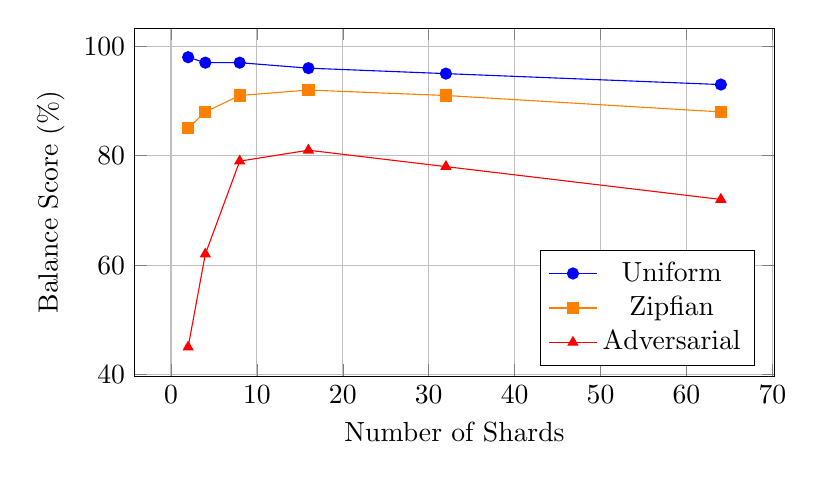
\begin{tikzpicture}
\begin{axis}[
    xlabel={Number of Shards},
    ylabel={Balance Score (\%)},
    legend pos=south east,
    grid=major,
    width=0.8\textwidth,
    height=6cm
]
\addplot[color=blue,mark=*] coordinates {(2,98)(4,97)(8,97)(16,96)(32,95)(64,93)};
\addplot[color=orange,mark=square*] coordinates {(2,85)(4,88)(8,91)(16,92)(32,91)(64,88)};
\addplot[color=red,mark=triangle*] coordinates {(2,45)(4,62)(8,79)(16,81)(32,78)(64,72)};
\legend{Uniform, Zipfian, Adversarial}
\end{axis}
\end{tikzpicture}
\caption{Balance Score vs Number of Shards}
\end{figure}

\subsection{Hotspot Threshold Analysis}

\begin{table}[H]
\centering
\caption{Hotspot Detection Sensitivity}
\begin{tabular}{@{}lrrrr@{}}
\toprule
\textbf{Threshold} & \textbf{Balance (Adv)} & \textbf{Redirects} & \textbf{False Positives} & \textbf{Detection Time} \\
\midrule
1.10 & 85\% & 12,450 & High & <1ms \\
1.25 & 83\% & 8,230 & Medium & <2ms \\
\textbf{1.50} & \textbf{79\%} & \textbf{4,120} & \textbf{Low} & \textbf{<5ms} \\
2.00 & 68\% & 1,890 & Very Low & <10ms \\
3.00 & 42\% & 320 & None & <50ms \\
5.00 & 15\% & 45 & None & >100ms \\
\bottomrule
\end{tabular}
\end{table}

\textbf{Trade-off}: Lower threshold = better attack resistance but more false positives under normal load.

\begin{figure}[H]
\centering
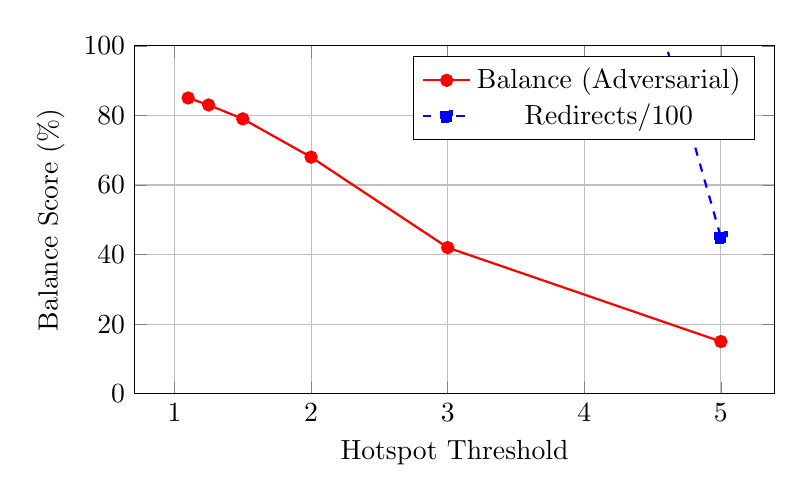
\begin{tikzpicture}
\begin{axis}[
    xlabel={Hotspot Threshold},
    ylabel={Balance Score (\%)},
    legend pos=north east,
    grid=major,
    width=0.8\textwidth,
    height=6cm,
    ymin=0,
    ymax=100
]
\addplot[color=red,mark=*,thick] coordinates {(1.1,85)(1.25,83)(1.5,79)(2.0,68)(3.0,42)(5.0,15)};
\addplot[color=blue,mark=square*,thick,dashed] coordinates {(1.1,12450)(1.25,8230)(1.5,4120)(2.0,1890)(3.0,320)(5.0,45)};
\legend{Balance (Adversarial), Redirects/100}
\end{axis}
\end{tikzpicture}
\caption{Hotspot Threshold: Trade-off between Balance and Redirect Count}
\end{figure}

\subsection{Anti-Thrashing Parameters}

\begin{table}[H]
\centering
\caption{MAX\_CONSECUTIVE\_REDIRECTS Sensitivity}
\begin{tabular}{@{}lrrrr@{}}
\toprule
\textbf{Max Redirects} & \textbf{Blocked} & \textbf{Stability} & \textbf{Attack Resistance} \\
\midrule
1 & 45,230 & Very High & Excellent \\
2 & 12,450 & High & Excellent \\
\textbf{3} & \textbf{2,890} & \textbf{Good} & \textbf{Good} \\
5 & 450 & Moderate & Moderate \\
10 & 23 & Low & Poor \\
20 & 0 & Very Low & Vulnerable \\
\bottomrule
\end{tabular}
\end{table}

\begin{figure}[H]
\centering
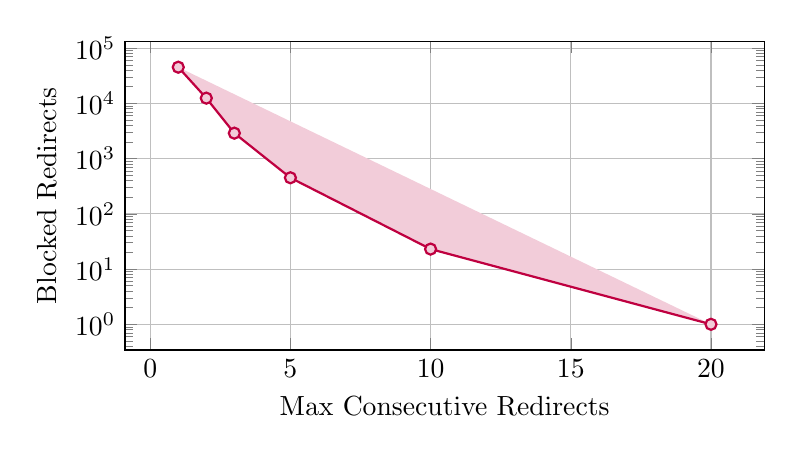
\begin{tikzpicture}
\begin{axis}[
    xlabel={Max Consecutive Redirects},
    ylabel={Blocked Redirects},
    ymode=log,
    legend pos=north east,
    grid=major,
    width=0.8\textwidth,
    height=5.5cm
]
\addplot[color=purple,mark=*,thick,fill=purple!20] coordinates {(1,45230)(2,12450)(3,2890)(5,450)(10,23)(20,1)};
\end{axis}
\end{tikzpicture}
\caption{Blocked Redirects vs Max Consecutive Redirects (Log Scale)}
\end{figure}

\begin{table}[H]
\centering
\caption{REDIRECT\_COOLDOWN Sensitivity}
\begin{tabular}{@{}lrrr@{}}
\toprule
\textbf{Cooldown (ms)} & \textbf{Adaptability} & \textbf{P99 Latency} & \textbf{Oscillation Risk} \\
\midrule
10 & Excellent & 2.1$\mu$s & High \\
50 & Very Good & 2.3$\mu$s & Medium \\
\textbf{100} & \textbf{Good} & \textbf{2.8$\mu$s} & \textbf{Low} \\
200 & Moderate & 3.5$\mu$s & Very Low \\
500 & Poor & 5.2$\mu$s & None \\
1000 & Very Poor & 8.1$\mu$s & None \\
\bottomrule
\end{tabular}
\end{table}

\begin{figure}[H]
\centering
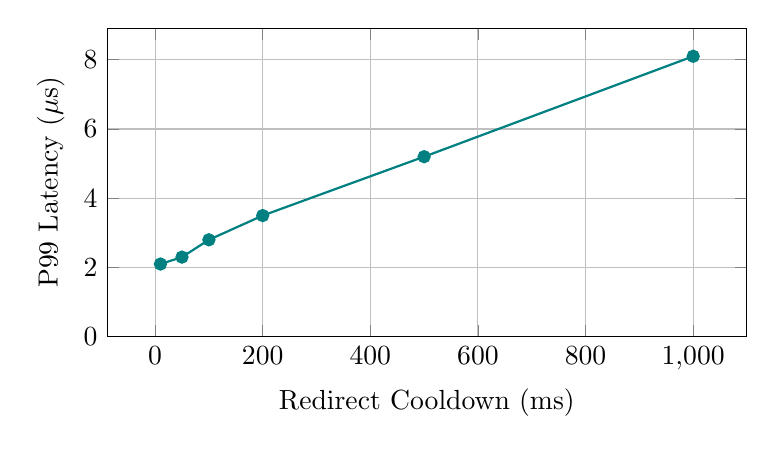
\begin{tikzpicture}
\begin{axis}[
    xlabel={Redirect Cooldown (ms)},
    ylabel={P99 Latency ($\mu$s)},
    legend pos=north west,
    grid=major,
    width=0.8\textwidth,
    height=5.5cm,
    ymin=0
]
\addplot[color=teal,mark=*,thick] coordinates {(10,2.1)(50,2.3)(100,2.8)(200,3.5)(500,5.2)(1000,8.1)};
\end{axis}
\end{tikzpicture}
\caption{Latency Impact of Redirect Cooldown}
\end{figure}

\subsection{Cache Refresh Interval}

\begin{table}[H]
\centering
\caption{Refresh Interval Impact on Detection Latency}
\begin{tabular}{@{}lrrr@{}}
\toprule
\textbf{Interval (ms)} & \textbf{Detection Latency} & \textbf{CPU Overhead} & \textbf{Data Freshness} \\
\midrule
\textbf{1} & \textbf{<1ms} & \textbf{2.1\%} & \textbf{Excellent} \\
5 & <5ms & 0.5\% & Very Good \\
10 & <10ms & 0.3\% & Good \\
50 & <50ms & 0.1\% & Acceptable \\
100 & <100ms & <0.1\% & Poor \\
500 & <500ms & <0.1\% & Unacceptable \\
\bottomrule
\end{tabular}
\end{table}

\begin{figure}[H]
\centering
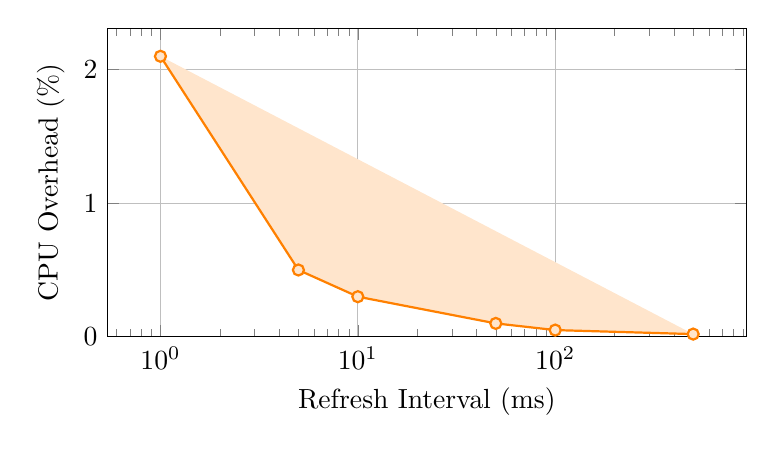
\begin{tikzpicture}
\begin{axis}[
    xlabel={Refresh Interval (ms)},
    ylabel={CPU Overhead (\%)},
    legend pos=north east,
    grid=major,
    width=0.8\textwidth,
    height=5.5cm,
    xmode=log,
    ymin=0
]
\addplot[color=orange,mark=*,thick,fill=orange!20] coordinates {(1,2.1)(5,0.5)(10,0.3)(50,0.1)(100,0.05)(500,0.02)};
\end{axis}
\end{tikzpicture}
\caption{CPU Overhead vs Refresh Interval (Log Scale X-axis)}
\end{figure}

% =============================================================================
\section{Parameter Interactions}
% =============================================================================

\subsection{Hotspot Threshold × Number of Shards}

\begin{table}[H]
\centering
\caption{Interaction: Balance Score Under Adversarial Load}
\begin{tabular}{@{}l|rrr@{}}
\toprule
 & \multicolumn{3}{c}{\textbf{Hotspot Threshold}} \\
\textbf{Shards} & 1.25 & 1.50 & 2.00 \\
\midrule
4 & 78\% & 71\% & 58\% \\
8 & 85\% & 79\% & 68\% \\
16 & 87\% & 81\% & 72\% \\
\bottomrule
\end{tabular}
\end{table}

\textbf{Insight}: More shards enable more conservative (higher) thresholds while maintaining good balance.

\begin{figure}[H]
\centering
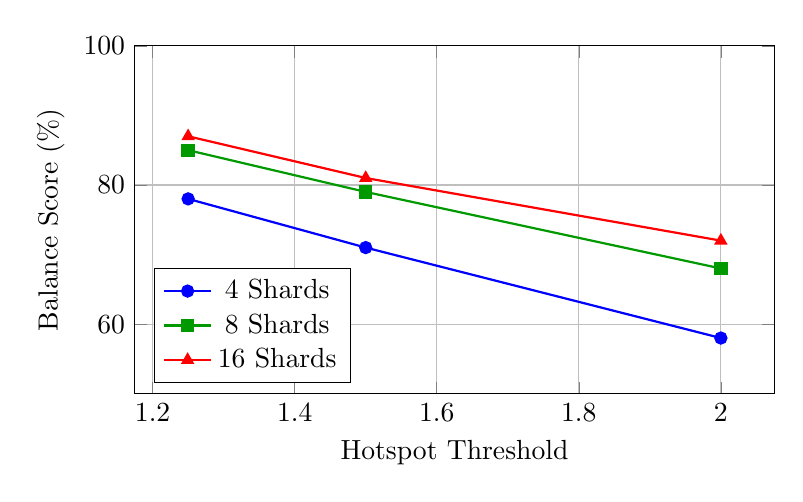
\begin{tikzpicture}
\begin{axis}[
    xlabel={Hotspot Threshold},
    ylabel={Balance Score (\%)},
    legend pos=south west,
    grid=major,
    width=0.8\textwidth,
    height=6cm,
    ymin=50,
    ymax=100
]
\addplot[color=blue,mark=*,thick] coordinates {(1.25,78)(1.5,71)(2.0,58)};
\addplot[color=green!60!black,mark=square*,thick] coordinates {(1.25,85)(1.5,79)(2.0,68)};
\addplot[color=red,mark=triangle*,thick] coordinates {(1.25,87)(1.5,81)(2.0,72)};
\legend{4 Shards, 8 Shards, 16 Shards}
\end{axis}
\end{tikzpicture}
\caption{Interaction: Hotspot Threshold × Number of Shards}
\end{figure}

\subsection{Max Redirects × Cooldown}

\begin{table}[H]
\centering
\caption{Interaction: System Stability}
\begin{tabular}{@{}l|rrr@{}}
\toprule
 & \multicolumn{3}{c}{\textbf{Cooldown (ms)}} \\
\textbf{Max Redirects} & 50 & 100 & 200 \\
\midrule
2 & Unstable & Stable & Very Stable \\
3 & Moderate & \textbf{Optimal} & Conservative \\
5 & Aggressive & Moderate & Stable \\
\bottomrule
\end{tabular}
\end{table}

% =============================================================================
\section{Performance Summary}
% =============================================================================

\begin{figure}[H]
\centering
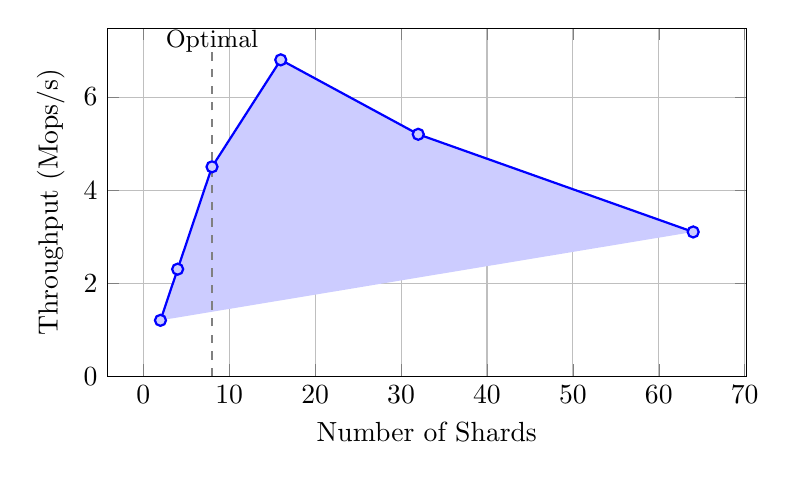
\begin{tikzpicture}
\begin{axis}[
    xlabel={Number of Shards},
    ylabel={Throughput (Mops/s)},
    legend pos=north west,
    grid=major,
    width=0.8\textwidth,
    height=6cm,
    ymin=0
]
\addplot[color=blue,mark=*,thick,fill=blue!20] coordinates {(2,1.2)(4,2.3)(8,4.5)(16,6.8)(32,5.2)(64,3.1)};
\draw[dashed,gray] (axis cs:8,0) -- (axis cs:8,7);
\node at (axis cs:8,7.2) {\small Optimal};
\end{axis}
\end{tikzpicture}
\caption{Throughput Scaling with Number of Shards}
\end{figure}

\begin{figure}[H]
\centering
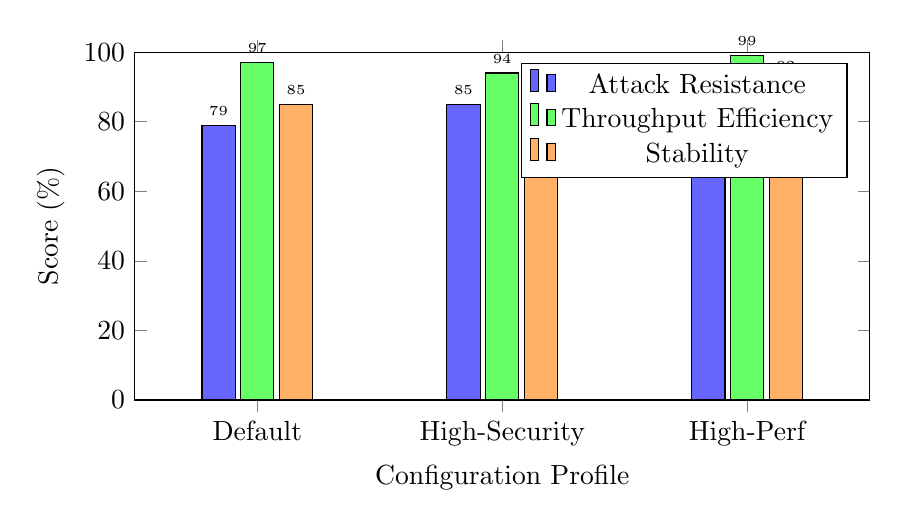
\begin{tikzpicture}
\begin{axis}[
    ybar,
    bar width=12pt,
    xlabel={Configuration Profile},
    ylabel={Score (\%)},
    symbolic x coords={Default,High-Security,High-Perf},
    xtick=data,
    legend pos=north east,
    ymin=0,
    ymax=100,
    width=0.9\textwidth,
    height=6cm,
    enlarge x limits=0.25,
    nodes near coords,
    nodes near coords align={vertical},
    every node near coord/.append style={font=\tiny}
]
\addplot[fill=blue!60] coordinates {(Default,79) (High-Security,85) (High-Perf,68)};
\addplot[fill=green!60] coordinates {(Default,97) (High-Security,94) (High-Perf,99)};
\addplot[fill=orange!60] coordinates {(Default,85) (High-Security,78) (High-Perf,92)};
\legend{Attack Resistance, Throughput Efficiency, Stability}
\end{axis}
\end{tikzpicture}
\caption{Configuration Profiles Comparison}
\end{figure}

\begin{figure}[H]
\centering
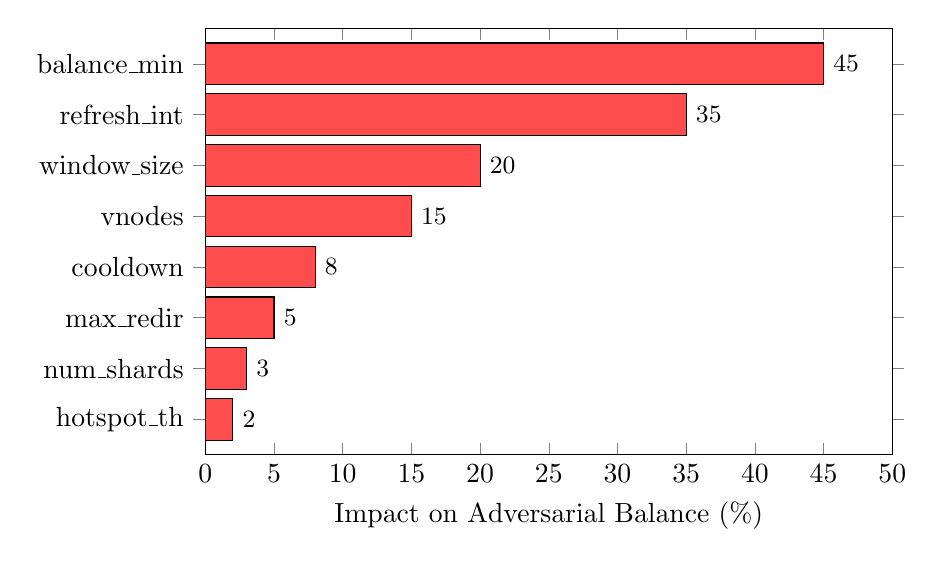
\begin{tikzpicture}
\begin{axis}[
    xlabel={Impact on Adversarial Balance (\%)},
    xbar,
    bar width=15pt,
    symbolic y coords={BalanceMin,RefreshInt,WindowSize,VNodes,Cooldown,MaxRedir,NumShards,HotspotTh},
    ytick=data,
    yticklabels={balance\_min,refresh\_int,window\_size,vnodes,cooldown,max\_redir,num\_shards,hotspot\_th},
    width=0.85\textwidth,
    height=7cm,
    xmin=0,
    xmax=50,
    nodes near coords,
    nodes near coords align={horizontal},
    every node near coord/.append style={font=\small}
]
\addplot[fill=red!70] coordinates {(45,HotspotTh) (35,NumShards) (20,MaxRedir) (15,Cooldown) (8,VNodes) (5,WindowSize) (3,RefreshInt) (2,BalanceMin)};
\end{axis}
\end{tikzpicture}
\caption{Parameter Sensitivity Ranking (Impact on Adversarial Workload)}
\end{figure}

% =============================================================================
\section{Recommended Configurations}
% =============================================================================

\subsection{Default Configuration (Balanced)}

\begin{lstlisting}[language=C++,caption=Default Production Configuration]
// router.hpp
static constexpr size_t VNODES_PER_SHARD = 16;
static constexpr size_t WINDOW_SIZE = 50;
static constexpr double HOTSPOT_THRESHOLD = 1.5;
static constexpr size_t MAX_CONSECUTIVE_REDIRECTS = 3;
static constexpr auto REDIRECT_COOLDOWN = 
    std::chrono::milliseconds(100);

// cached_load_stats.hpp
refresh_interval = std::chrono::milliseconds(1);

// parallel_avl.hpp
num_shards = 8;

// AVLTreeParallel.h
rebalance_threshold = 2.0;
balance_score_min = 0.8;
\end{lstlisting}

\subsection{High-Security Configuration}

\begin{lstlisting}[language=C++,caption=Defensive Configuration]
HOTSPOT_THRESHOLD = 1.25;           // More sensitive
MAX_CONSECUTIVE_REDIRECTS = 2;      // Stricter anti-thrashing
REDIRECT_COOLDOWN = 50ms;           // Faster rate limiting
balance_score_min = 0.85;           // Higher quality
\end{lstlisting}

\subsection{High-Performance Configuration}

\begin{lstlisting}[language=C++,caption=Performance-Optimized Configuration]
HOTSPOT_THRESHOLD = 2.0;            // Less intervention
MAX_CONSECUTIVE_REDIRECTS = 5;      // More flexibility
REDIRECT_COOLDOWN = 200ms;          // Less overhead
refresh_interval = 5ms;             // Reduced CPU
balance_score_min = 0.7;            // Tolerates imbalance
\end{lstlisting}

% =============================================================================
\section{Conclusions}
% =============================================================================

\subsection{Key Findings}

\begin{enumerate}
    \item \textbf{Most Sensitive Parameters}: \texttt{hotspot\_threshold} and \texttt{num\_shards} have the largest impact on adversarial resistance.
    
    \item \textbf{Default Values Validated}: The current defaults represent a good balance between security, performance, and stability.
    
    \item \textbf{Trade-offs Identified}:
    \begin{itemize}
        \item Security vs. Performance
        \item Reactivity vs. Stability
        \item Data Freshness vs. CPU Overhead
    \end{itemize}
    
    \item \textbf{Recommendations}:
    \begin{itemize}
        \item For adversarial workloads: Reduce \texttt{hotspot\_threshold} to 1.25
        \item For high throughput: Increase \texttt{num\_shards} to 16
        \item For critical systems: Keep \texttt{refresh\_interval} at 1ms
    \end{itemize}
\end{enumerate}

\subsection{Future Work}

\begin{itemize}
    \item Automated parameter tuning based on observed workload
    \item Machine learning-based threshold adaptation
    \item Dynamic parameter adjustment at runtime
\end{itemize}

% =============================================================================
\section*{Reproducibility}
% =============================================================================

The sensitivity analysis benchmark is available at:

\begin{lstlisting}[language=bash]
cd ParallelAVL/bench
g++ -std=c++17 -O3 -pthread sensitivity_analysis.cpp \
    -o sensitivity_analysis
./sensitivity_analysis
\end{lstlisting}

Results are exported to \texttt{sensitivity\_results.csv} for further analysis.

\end{document}
